\section{Tighly Integrated Building Information System Architecture}

The first building information systems became commericially available in the 1970's ~\cite{gardner1987energy}.  
Historically, building management 
systems were constructed as a collection of control loops, which progressed from pneumatic to analog to digital.
These control loops largely form the foundation for the design decisions made in building information systems.  
This section gives a quick overview of the architecture bottom-up and describes how each stage is built around
the concept of loops and supervisory control.  We then describe some of the short-comings of this architecture
and give an overview of how we address it in a system called StreamFS -- described in more details in
the remaining chapters.

\begin{figure}[t!] %htbp
\centering
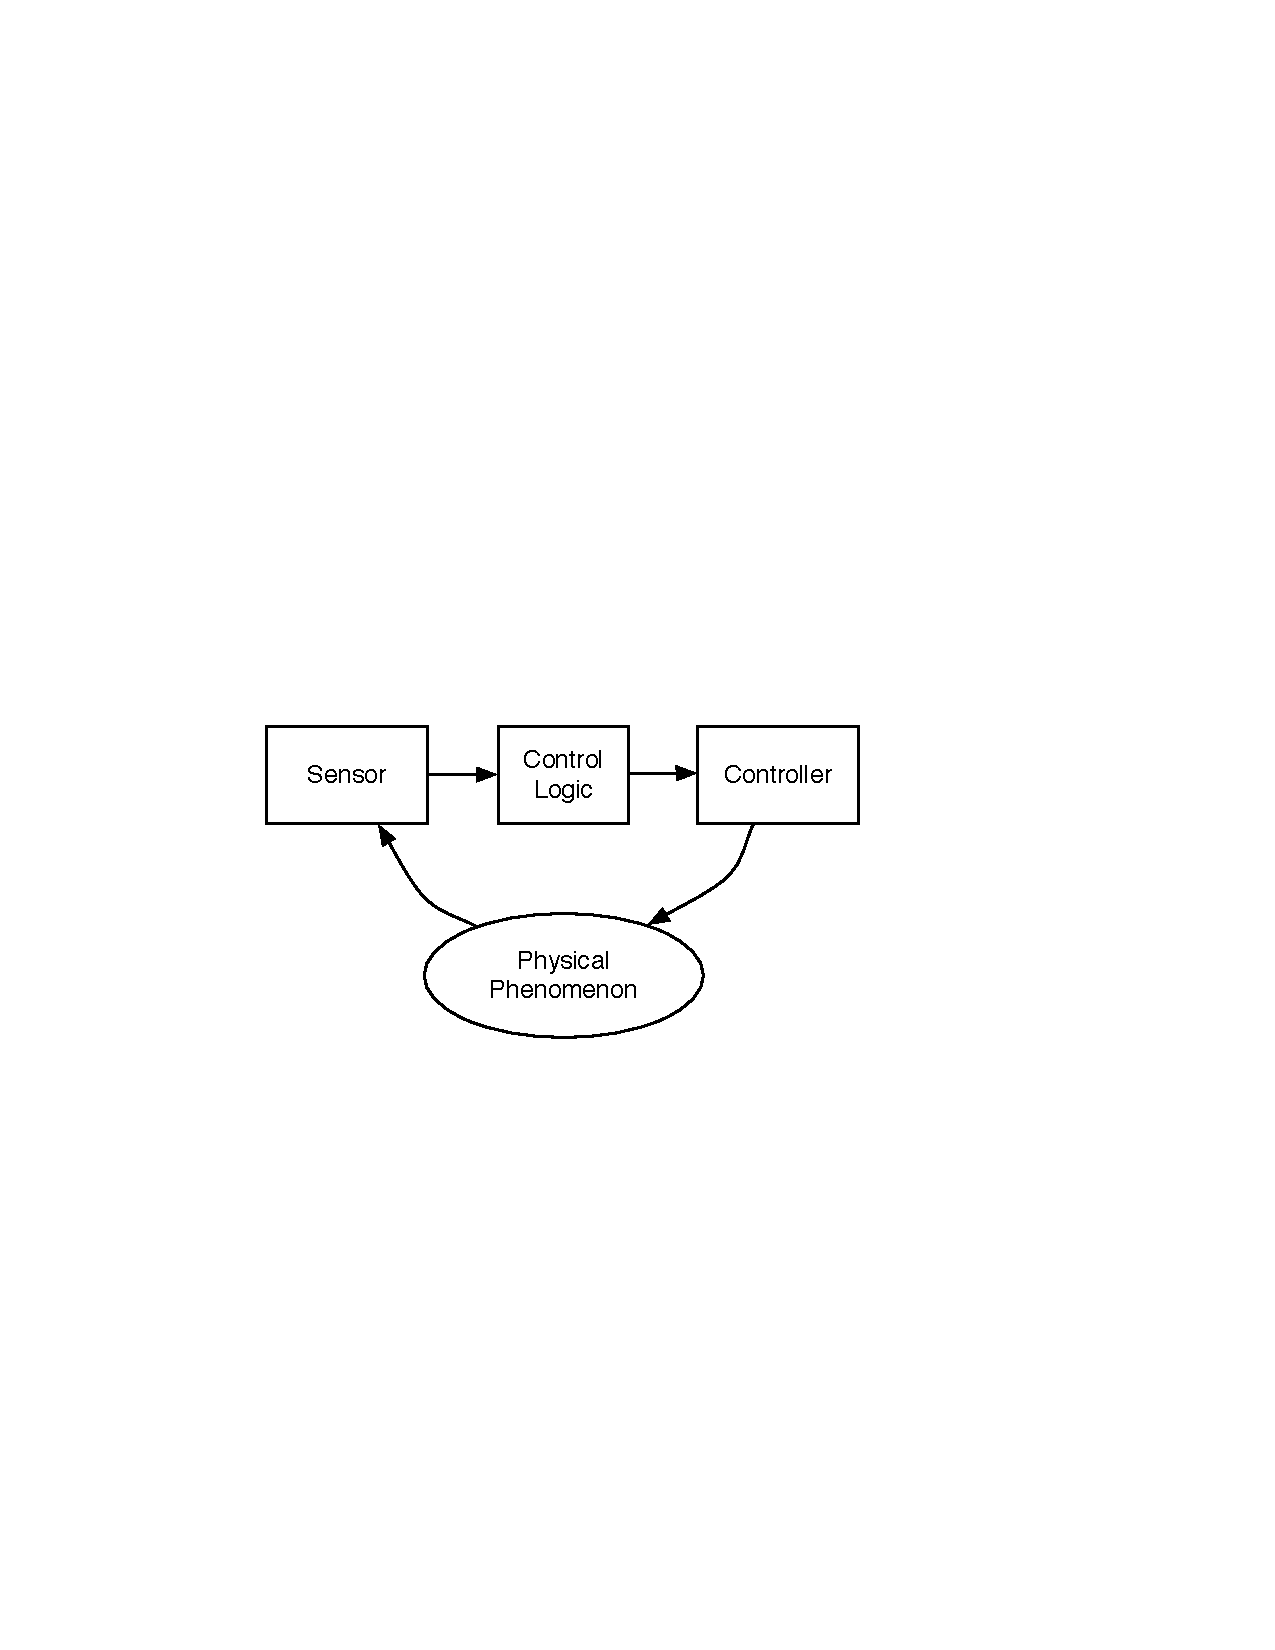
\includegraphics[width=0.50\columnwidth]{figs/control_loop}
\caption{General building control loop.}
\label{fig:control_loop}
\end{figure}

\subsection{Control Loops and The Outstation}
\label{sec:control_loops}
Each loop is defined by a control domain consisting of a sensor, an actuator, and a control mechanism.  The control mechanism
become logic based when signals from sensors moved to the digital domain.  However, the basic control principal was based
entirely on local control loops, with the implicit assumption that these loops were largely independent of one another.
Figure~\ref{fig:control_loop} shows a high-level control loop.  For example, the temperature control loop has a temperature
sensor as the input and uses the temperature set-point parameter to decide when and which actuators to activate.
For temperature control this actuation controls the the valve that lets cool air into the space.  This causes the temeprature
to fall until a lower-bound is reached and the control logic is activated again.

The figure also shows the basic structure inside an outstation.  An outstation is a box that contains up to several control boards, each
wired to one or more sensors and one or more actuators.  The outstation is typically close to the sensors and actuators (in the same room)
and contains all the control logic for the local plant.  Inside the control logic there is a CPU and some memory.  The memory
contains the control program and some space for sensor readings.  It is directly wired to the sensors and actuators through
a series of buses and shown in Figure~\ref{fig:control_box}.

\begin{figure}[t!] %htbp
\centering
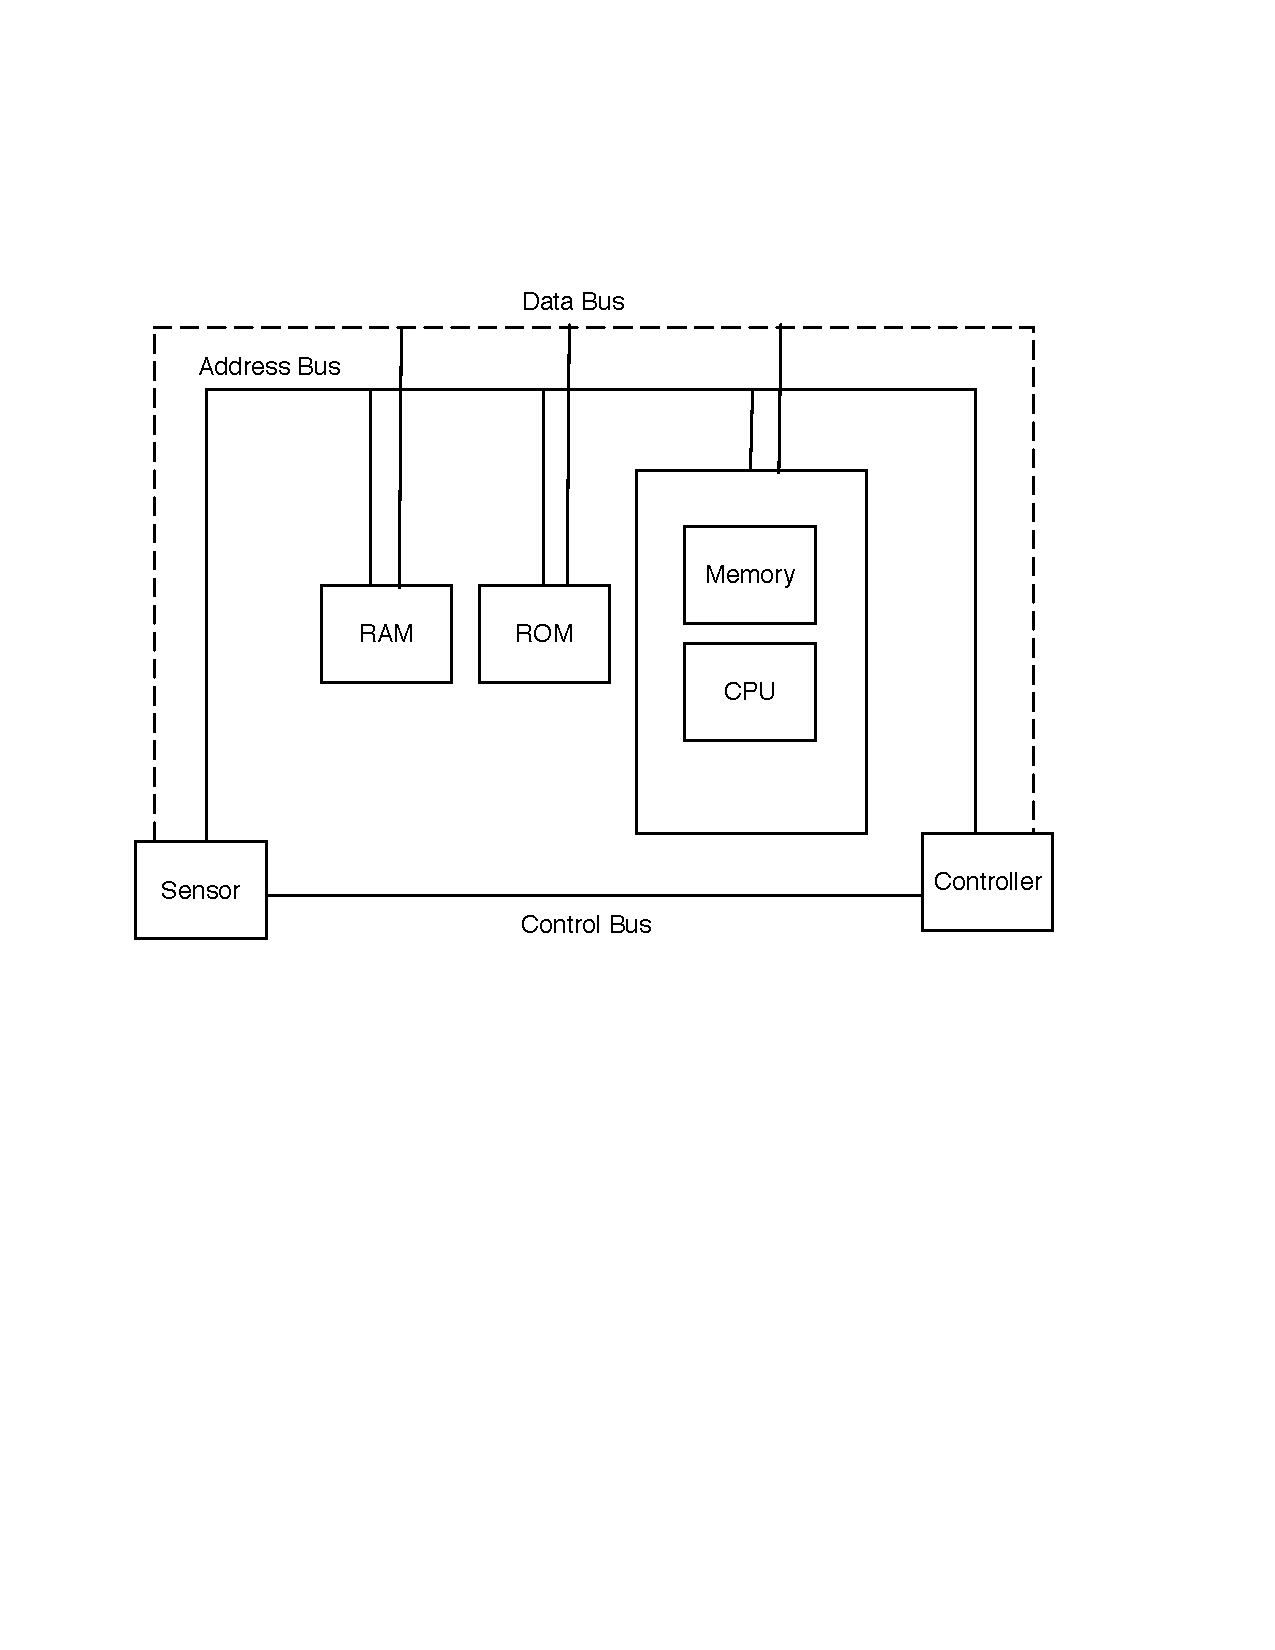
\includegraphics[width=0.50\columnwidth]{figs/control_box}
\caption{High-level control board architecture.}
\label{fig:control_box}
\end{figure}

As readings from the sensors are taken, they are placed in RAM.  The amount of RAM is limited and can get filled up, so it is important
to schedule periodic collection tasks from the central station -- the building management system (BMS).  The control logic is typically
written in ROM and can only be changed by the vendor.  The input parameters are set at the BMS and they dedicate the operational dynamics
of the control scheme in reaction to the input~\cite{BMS_book}.
Outstations are distributed through the building and are essentially running independent of one another.  In order to enable centralized 
monitoring and control, they are networked together and report some of the sensor readings and control-logic state to a central outstation.

\subsection{Central Outstation and Communication Protocols}
The central outstation is typically a Microsoft Windows-based PC connected to the outstation through either RS-485/modbus or ethernet.
The user interacts with the system through a graphical interface, constructed from the schematics for the building or the schematics
for the component in the system that is being monitored.  The BMS running on the PC communicates with the outstations through either a 
proprietary protocol or an open one like BACNet~\cite{Bacnet} or LonTalk~\cite{LonTalk}.

\begin{figure}[h!] %htbp
\centering
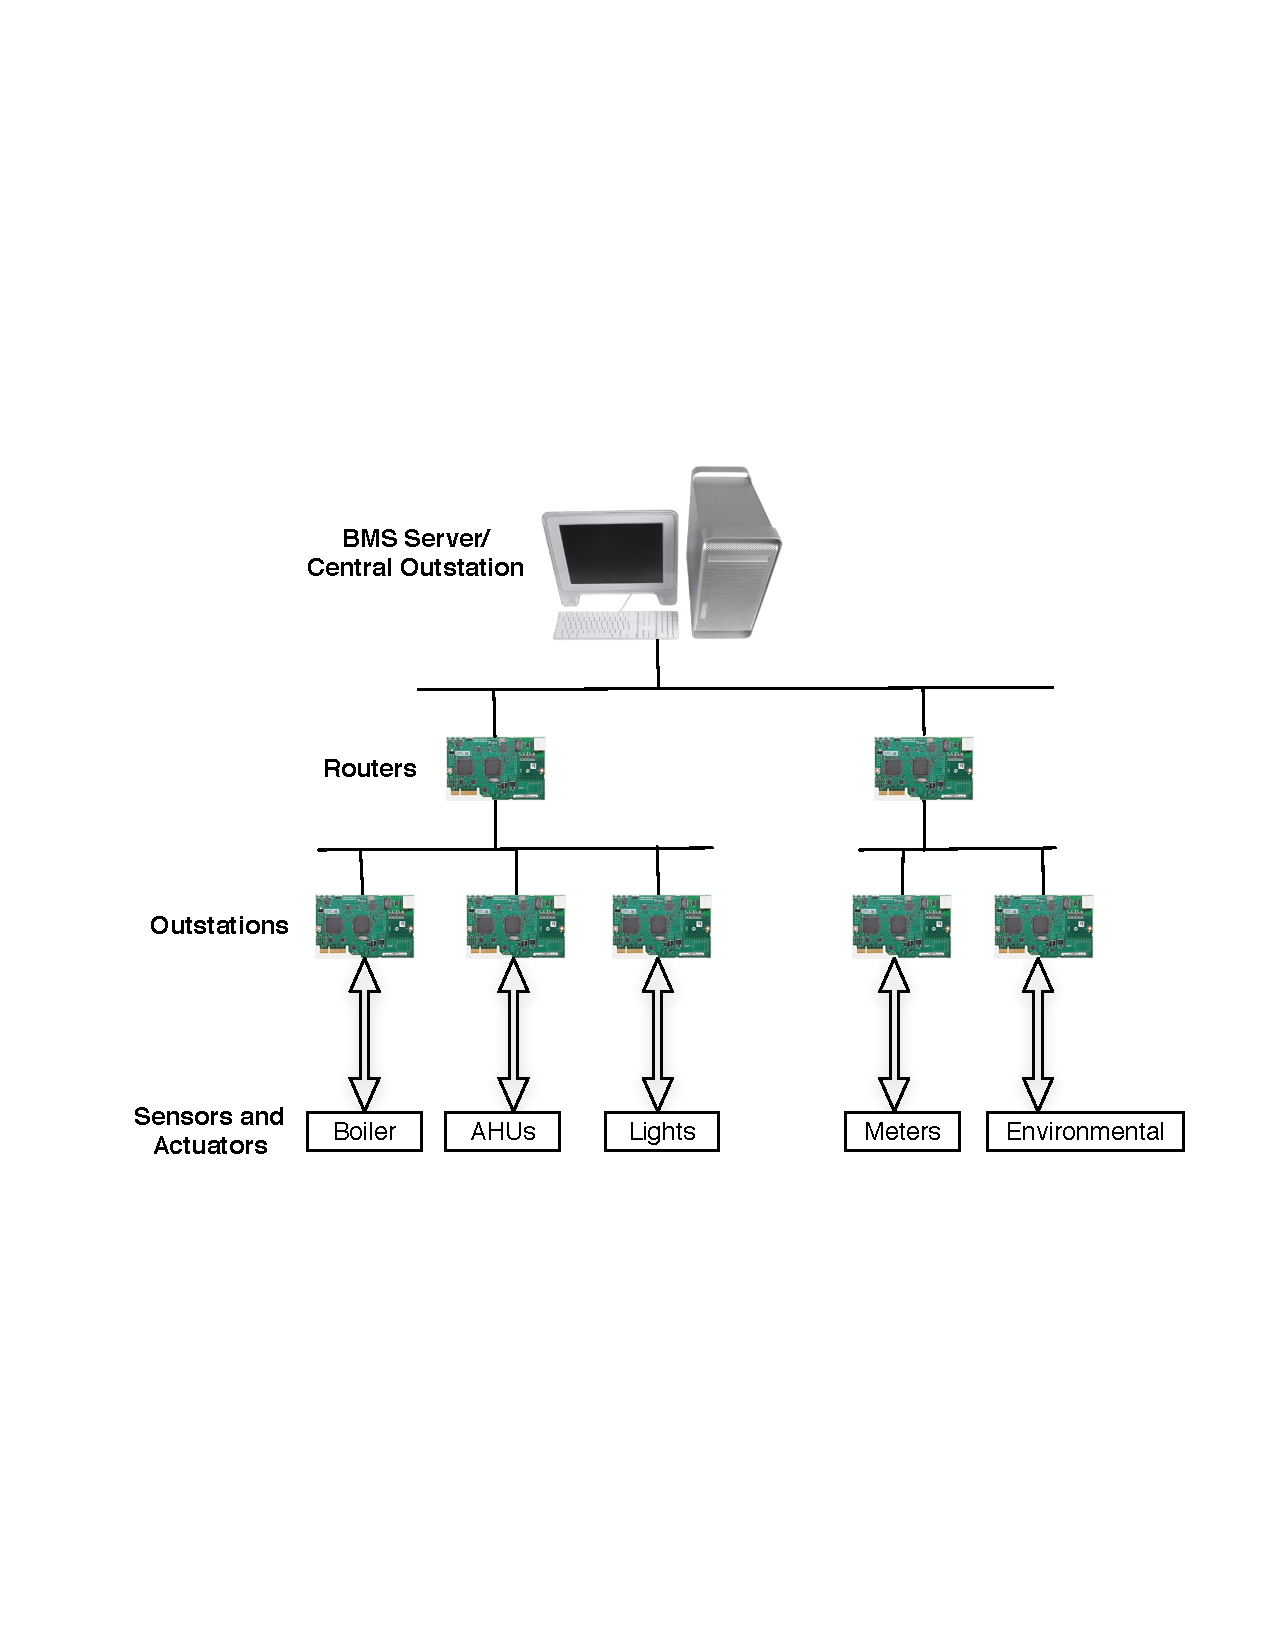
\includegraphics[width=0.50\columnwidth]{figs/BMS_network}
\caption{High-level control board architecture.}
\label{fig:bms_network}
\end{figure}

Both protocols define both a wire protocol and packet structure for communicating with the outstations.  From these there's a high-level
structure for the individual points throughout the system.  A point is a sensor/actuator or another kind of object, like a schedule object.
BACNet exposes the notion of devices as a collection of different types of objects.  Each object contains a set of properties that can 
be read and/or written.  A device is identifyable through a name or address on the network, each object has a unique identifier and is one of
many types -- such as input, output, value, analog, and many others~\cite{Bacnet}.  

These protocols also provide a protocol for discovery and read/write.  Each [device, object name/id, property name/id] tuple forms a name.
This name is typically what is exposed by the protocol to the application.  All the names are set by the vendor and the graphical interface, 
constructed from the building schematics, is also designed and constructed by the vendor.  The building manger is the primary user of the system,
so rather than expose the underlying protocol, he/she interacts with the building via the graphical interface.

In order to interact with the underlying sensor and actuator layer, the application must use a stub that communicates directly with the 
sensor/actuator through the BACnet stack.  Services treated similarly to sensors/actuators.  They are represented as a collection of 
objects with readable/writable properties.  An example service that is provided in BACNet is  \emph{WhoIs} and \emph{EventNotification}.
The former is a broadcast service that is used for discovery of other objects, the latter is used for setting alarms on the sensor data that
are reported by the BACNet enabled devices on the network in the outstation layer.  There are many other types of events that are supported 
and over 50 types of object types in the baseline protocol, which is extensible.  Device and object names that are added have no restriction
on either the number of characters (specified by the vendor) or the encoding.


\begin{figure}[t!] %htbp
\centering
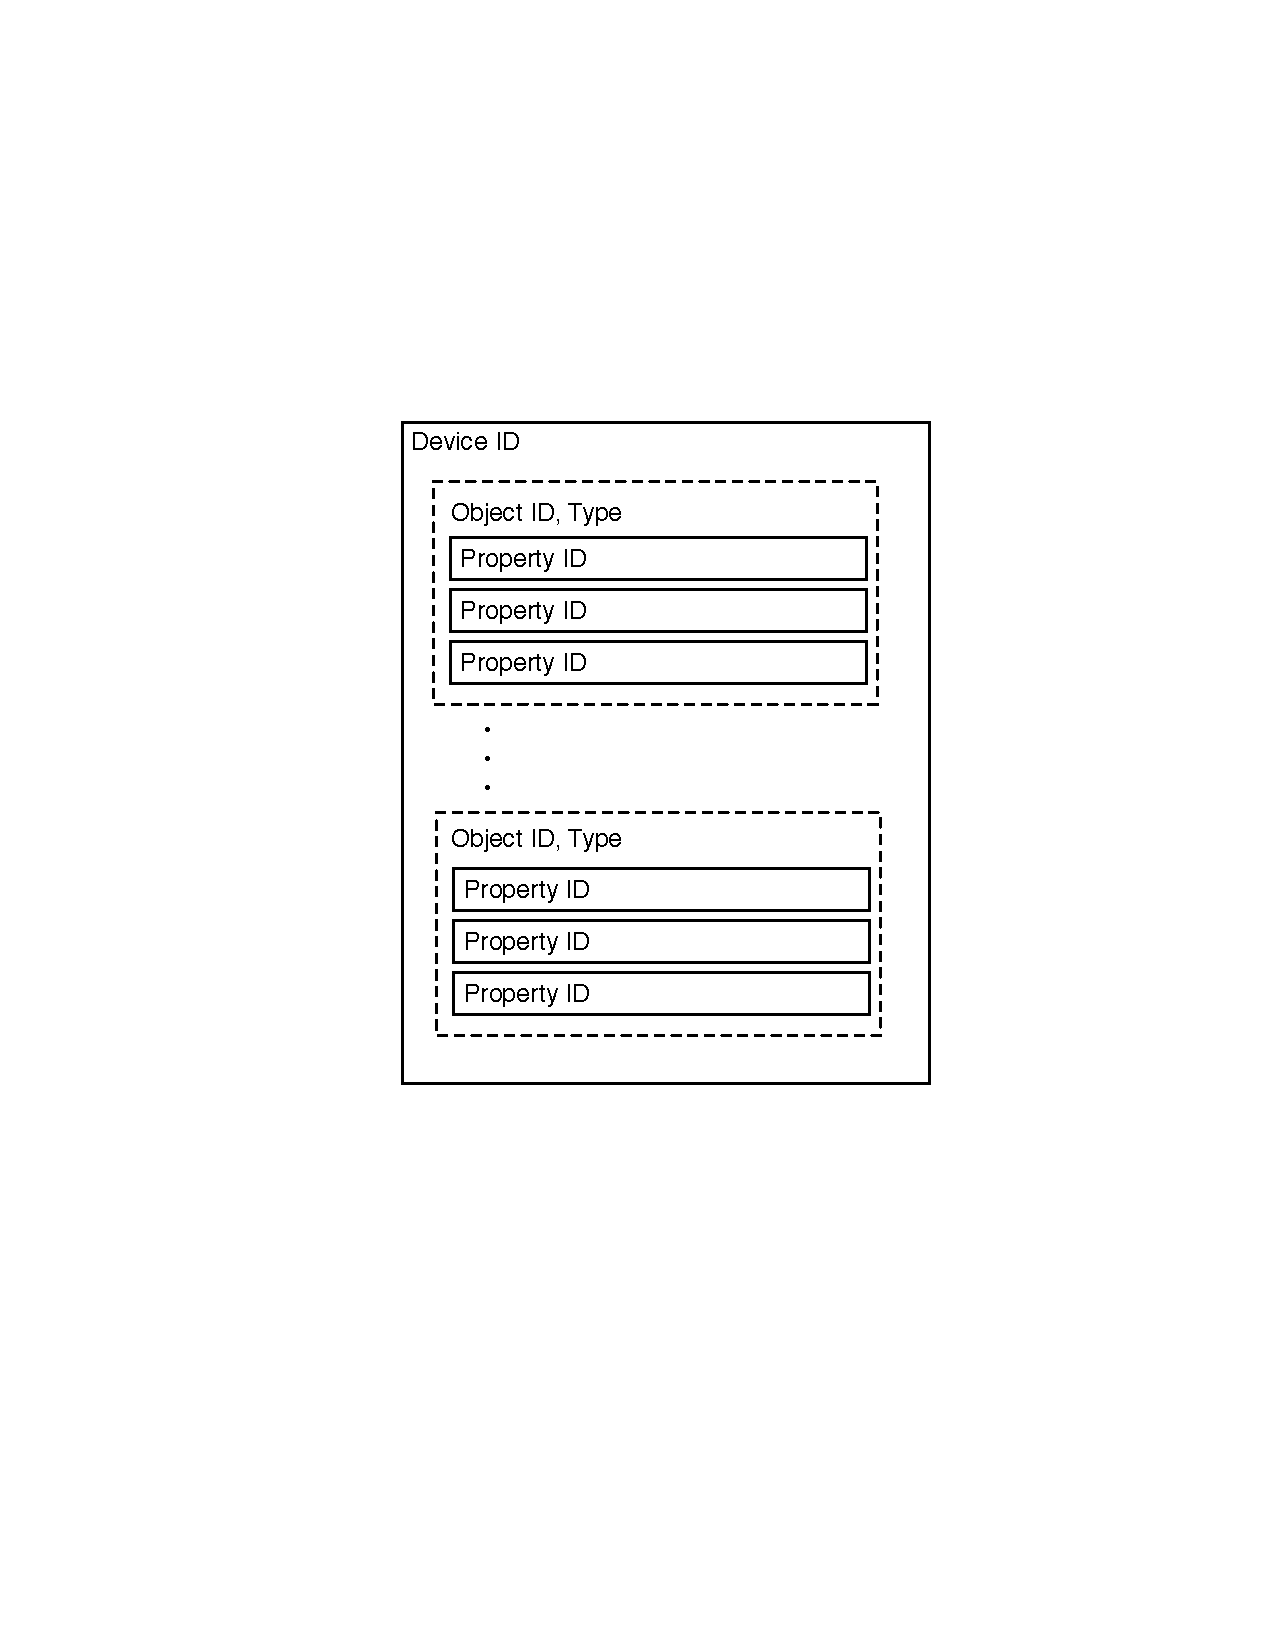
\includegraphics[width=0.25\columnwidth]{figs/bacnet_device}
\caption{BACNet device example.}
\label{fig:bacnet_device}
\end{figure}